% PHY 210 Math Pretest, Fall 2026 -- Michael Lerner, Smith College
%
% Ported 2026-08-17 from the S23/S26 pretest (Casey Berger's LaTeX source,
% reused by Gillian Beltz-Mohrmann / Manbir Kaur in S26; descended from Gary
% Felder's pretest). Figures regenerated from scratch (make_pretest_figures.py).
% Changes from the S26 version:
%   - Problem 3b: restored y(t) = t^2 + 1 and wrote df/dt (the S23/S26
%     statement omitted y(t) and wrote partial f/partial t, but the posted
%     solutions solve the full chain rule WITH y(t) = t^2 + 1 -- the statement
%     and solutions disagreed; this matches the solutions and the intent).
%   - "Mathematica" -> computer tools generally (we use Python).
%   - Solutions included inline via \answer{}, hidden in the student build.
%
% BUILD (from this directory):
%   student: pdflatex -jobname=MathPretest-student "\def\STUDENTVERSION{}% PHY 210 Math Pretest, Fall 2026 -- Michael Lerner, Smith College
%
% Ported 2026-08-17 from the S23/S26 pretest (Casey Berger's LaTeX source,
% reused by Gillian Beltz-Mohrmann / Manbir Kaur in S26; descended from Gary
% Felder's pretest). Figures regenerated from scratch (make_pretest_figures.py).
% Changes from the S26 version:
%   - Problem 3b: restored y(t) = t^2 + 1 and wrote df/dt (the S23/S26
%     statement omitted y(t) and wrote partial f/partial t, but the posted
%     solutions solve the full chain rule WITH y(t) = t^2 + 1 -- the statement
%     and solutions disagreed; this matches the solutions and the intent).
%   - "Mathematica" -> computer tools generally (we use Python).
%   - Solutions included inline via \answer{}, hidden in the student build.
%
% BUILD (from this directory):
%   student: pdflatex -jobname=MathPretest-student "\def\STUDENTVERSION{}% PHY 210 Math Pretest, Fall 2026 -- Michael Lerner, Smith College
%
% Ported 2026-08-17 from the S23/S26 pretest (Casey Berger's LaTeX source,
% reused by Gillian Beltz-Mohrmann / Manbir Kaur in S26; descended from Gary
% Felder's pretest). Figures regenerated from scratch (make_pretest_figures.py).
% Changes from the S26 version:
%   - Problem 3b: restored y(t) = t^2 + 1 and wrote df/dt (the S23/S26
%     statement omitted y(t) and wrote partial f/partial t, but the posted
%     solutions solve the full chain rule WITH y(t) = t^2 + 1 -- the statement
%     and solutions disagreed; this matches the solutions and the intent).
%   - "Mathematica" -> computer tools generally (we use Python).
%   - Solutions included inline via \answer{}, hidden in the student build.
%
% BUILD (from this directory):
%   student: pdflatex -jobname=MathPretest-student "\def\STUDENTVERSION{}% PHY 210 Math Pretest, Fall 2026 -- Michael Lerner, Smith College
%
% Ported 2026-08-17 from the S23/S26 pretest (Casey Berger's LaTeX source,
% reused by Gillian Beltz-Mohrmann / Manbir Kaur in S26; descended from Gary
% Felder's pretest). Figures regenerated from scratch (make_pretest_figures.py).
% Changes from the S26 version:
%   - Problem 3b: restored y(t) = t^2 + 1 and wrote df/dt (the S23/S26
%     statement omitted y(t) and wrote partial f/partial t, but the posted
%     solutions solve the full chain rule WITH y(t) = t^2 + 1 -- the statement
%     and solutions disagreed; this matches the solutions and the intent).
%   - "Mathematica" -> computer tools generally (we use Python).
%   - Solutions included inline via \answer{}, hidden in the student build.
%
% BUILD (from this directory):
%   student: pdflatex -jobname=MathPretest-student "\def\STUDENTVERSION{}\input{MathPretest.tex}"
%   master:  pdflatex -jobname=MathPretest-master MathPretest.tex
%
\documentclass[12pt]{article}
%%%%%%%%%%%%%%%%%%%%%%%%%%%%%%%%%%%%%%%%%%%%%%%%%%%%%%%%%%%%%
\input{../../macros}
%%%%%%%%%%%%%%%%%%%%%%%%%%%%%%%%%%%%%%%%%%%%%%%%%%%%%%%%%%%%%
% macros.tex defaults to \mastertrue; a student build passes \STUDENTVERSION.
\ifdefined\STUDENTVERSION \masterfalse \else \mastertrue \fi

\usepackage{graphicx}
\usepackage{enumitem}
\newcommand{\degs}{^{\circ}}
% macros.tex makes top-level enumerates lettered; this doc numbers its
% problems 1-9 with lettered subparts.
\renewcommand{\labelenumi}{\arabic{enumi}.}

\pagestyle{empty}
\begin{document}

\begin{center}
{\bf PHY 210: Mathematical Methods of Physical Sciences and Engineering\\
Smith College, Fall 2026}
\end{center}

\setlength{\unitlength}{1in}
\begin{picture}(6,.1)
\put(0,0) {\line(1,0){6.25}}
\end{picture}

\vskip.15in
\begin{center}
{\Large \bf Math Pretest}\\[2pt]
% Due date confirmed 2026-09-02 against the F2026 calendar (EXTRA_DUE) and
% the Moodle assignment: Fri Sep 18, 22:00. Same Friday as WHW02, as in S26.
{Due: Friday, September 18, end of day}
\end{center}

\subsection*{Instructions}
Set aside two hours for this pretest.

Please don't use a calculator, a computer, or any references. This pretest is
meant to give both of us a clear picture of which areas you should practice
more, so it won't help you to look things up. It is graded for completion, not
correctness: doing it thoughtfully is what earns the credit.

Give your answers as expressions. For example, if your final answer to a
question is $\sqrt{10}$, you should leave it as $\sqrt{10}$. If you have
something that can easily be simplified, like $e^{0}$ or $\ln(1)$, you should
simplify it.

\begin{enumerate}
  \item Write the equation of a line with slope $-5$ that passes through the
        point $(-2,2)$.
  \answer{Point-slope form: $y - 2 = -5(x+2)$, i.e.\ $y = -5x - 8$.
  Check: $x=-2$ gives $y=2$. \checkmark}

  \item Find the slope and concavity of $f(x) = x^{3} - x$ at $x=2$.
  \answer{$f'(x) = 3x^2 - 1$ and $f''(x) = 6x$, so at $x=2$ the slope is
  $f'(2) = 11$ and the concavity is $f''(2) = 12$ (concave up).}

  \item Calculate the following derivatives:
  \begin{enumerate}[label = \alph*.]
    \item $\pd{f}{y}$ for $f(x,y) = e^{3 x \sin(ky)}$
    \answer{$\pd{f}{y} = 3kx\cos(ky)\, e^{3x\sin(ky)}$.}
    \item $\fd{f}{t}$ for $f(x,y) = x^{3}e^{y}$, with $x(t) = \cos(2t)$ and
          $y(t) = t^{2} + 1$
    \answer{Chain rule:
    $\fd{f}{t} = \pd{f}{x}\fd{x}{t} + \pd{f}{y}\fd{y}{t}
               = 3x^2 e^y \left(-2\sin 2t\right) + x^3 e^y (2t)
               = 2t\cos^3(2t)\,e^{t^2+1} - 6\sin(2t)\cos^2(2t)\,e^{t^2+1}$.}
  \end{enumerate}

  \item Evaluate the following integrals:
  \begin{enumerate}[label = \alph*.]
    \item $\displaystyle\int \sin(x)\, [2 \cos(x) + 3]^{5}\,dx$
    \answer{Let $u = 2\cos x + 3$, $du = -2\sin x\,dx$:
    $-\tfrac{1}{2}\int u^5\,du = -\tfrac{1}{12}(2\cos x + 3)^6 + C$.}
    \item Integrate $f(x,y) = x-y$ over the triangular region shown below.

    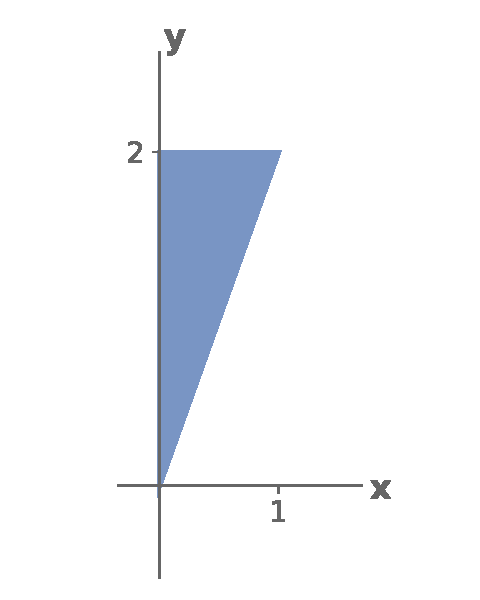
\includegraphics[width = 0.32\linewidth]{triangular_region}
    \answer{The slanted edge is the line $y = 2x$. Integrating $y$ first:
    $\int_0^1\!\!\int_{2x}^{2} (x-y)\,dy\,dx
     = \int_0^1 \left[xy - \tfrac{y^2}{2}\right]_{2x}^{2} dx
     = \int_0^1 (2x - 2)\,dx = -1$.
    (Integrating $x$ first, $\int_0^2\!\int_0^{y/2}(x-y)\,dx\,dy$, also gives
    $-1$.)}
  \end{enumerate}

  \item The point $P$ in the $x$-$y$ plane has Cartesian coordinates
        $x=-2,\ y=-2$. What are its polar coordinates $\rho$ and $\phi$?
        (You may have learned these as $r$ and $\theta$ --- they mean the
        same thing.)
  \answer{Draw it: $P$ is in the third quadrant.
  $\rho = \sqrt{(-2)^2 + (-2)^2} = 2\sqrt{2}$ and
  $\phi = \pi + \pi/4 = 5\pi/4$ (i.e.\ $225\degs$).}

  \item The plot below shows a function $f(x)$. On the axes provided at the
        right, sketch the function $df/dx$. Numbers are included on the
        horizontal axis, but you do not need to show numbers on the vertical
        axis.

  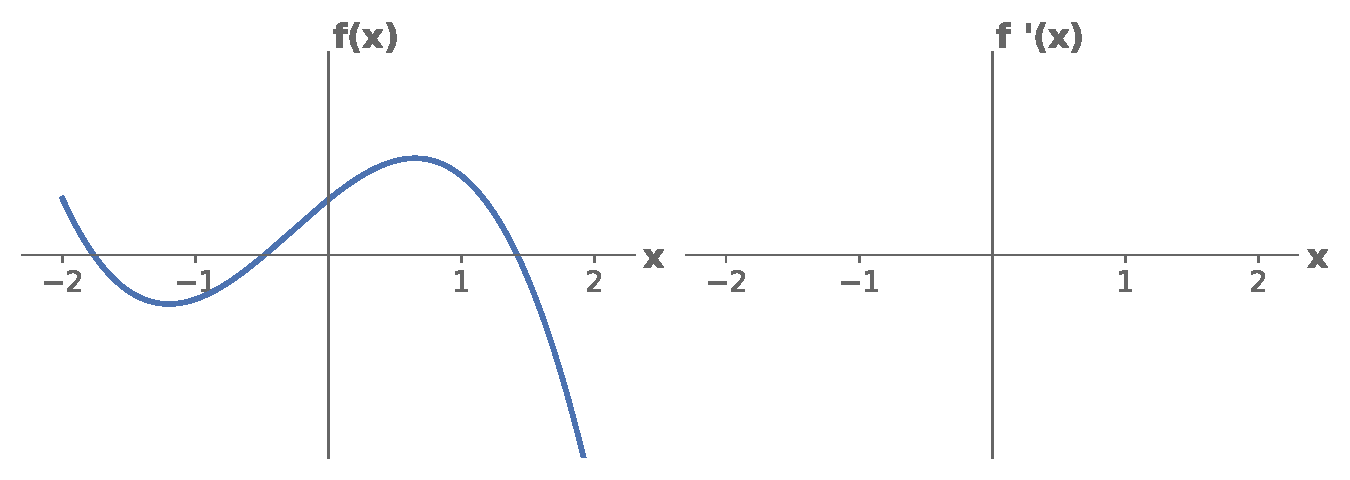
\includegraphics[width = \linewidth]{plotting_derivative}
  \answer{Where $f$ has its minimum (just before $x=-1$) and its maximum
  (between $0$ and $1$), $f' = 0$. To the left of the minimum and to the right
  of the maximum, $f$ is decreasing, so $f' < 0$; between them $f$ is
  increasing, so $f' > 0$. The sketch is a downward-opening arch crossing zero
  just before $x=-1$ and again between $0$ and $1$, negative and falling
  steeply at the right edge.}

  \item The plot below shows a cosine function $x(t)$.
  \begin{enumerate}[label = \alph*.]
    \item What are the amplitude $A$, period $T$, and angular frequency
          $\omega$?
    \item Write the function $x(t)$. {\em Hint: try plugging some points into
          your answer to make sure it matches the graph.}
  \end{enumerate}
  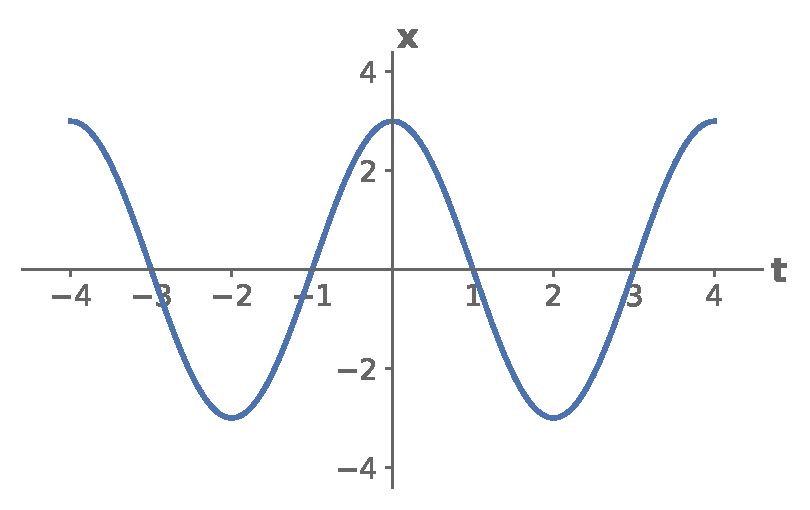
\includegraphics[width = 0.5\linewidth]{cosine_plot}
  \answer{$A = 3$ (the curve runs from $-3$ to $3$); $T = 4$ (peak to
  peak); $\omega = 2\pi/T = \pi/2$. So $x(t) = 3\cos(\pi t/2)$. Check:
  $x(0)=3$, $x(1)=0$, $x(2)=-3$, $x(4)=3$. \checkmark}

  \item The vector $\vA$ is given by
        $\vA = -2\hx + 5\hy$. The vector $\vB$ has magnitude $2\sqrt{2}$ and
        direction $30\degs$ clockwise from the positive $x$ axis.
  \begin{enumerate}[label = \alph*.]
    \item Find the magnitude and direction of $\vA$.
    \answer{$\abs{\vA} = \sqrt{4+25} = \sqrt{29}$. Draw it: $\vA$ points up
    and to the left, an angle $\tan^{-1}(2/5)$ counterclockwise from the
    positive $y$ axis (equivalently $\tan^{-1}(5/2)$ up from the negative $x$
    axis).}
    \item Find the components of $\vB$.
    \answer{$B_x = 2\sqrt{2}\cos(30\degs) = \sqrt{6}$,
    $B_y = -2\sqrt{2}\sin(30\degs) = -\sqrt{2}$ (negative: $30\degs$
    \emph{clockwise} is below the axis).}
    \item Find $\vA \cdot \vB$.
    \answer{$\vA\cdot\vB = A_x B_x + A_y B_y
    = -2\sqrt{6} - 5\sqrt{2}$. Sanity check: the vectors point mostly away
    from each other, so a negative answer makes sense.}
  \end{enumerate}

  \item An object is moving in some complicated way, and you want to solve
        for its acceleration at some particular moment. You can't actually do
        that calculation here, because we're not giving you enough
        information. Instead, check each of the following possible answers to
        determine whether it has correct units. Assume that:
  \begin{itemize}
    \item $F_{1}, F_{2}$, and so on are forces,
    \item $m$ is a mass,
    \item $D$ is a distance,
    \item $T$ is a time,
    \item $v_{0}$ and $v_{f}$ are speeds.
  \end{itemize}
  Which of the following possible answers have correct units? (There may be
  more than one option with correct units.)
  \begin{enumerate}[label = \alph*.]
    \item $a = \dfrac{v_{0} + v_{f}}{T}$
    \item $a = \dfrac{v_{0} + v_{f} + 1}{T}$
    \item $a = \dfrac{D}{T^{2}}$
    \item $a = \dfrac{D}{T^{2}}\,e^{-v_{f}/v_{0}}$
    \item $a = \dfrac{D}{T^{2}}\,e^{-v_{f}/(D T)}$
  \end{enumerate}
  \answer{Acceleration needs units of distance over time squared.
  (a) speed/time \checkmark\ YES.
  (b) NO --- you can't add a speed and the unitless number 1.
  (c) \checkmark\ YES.
  (d) the exponent is speed/speed, which is unitless, so \checkmark\ YES.
  (e) NO --- the exponent has units of $1/(\text{time})^2$, and exponents
  must be unitless.
  Correct units: a, c, and d.}
\end{enumerate}

\end{document}
"
%   master:  pdflatex -jobname=MathPretest-master MathPretest.tex
%
\documentclass[12pt]{article}
%%%%%%%%%%%%%%%%%%%%%%%%%%%%%%%%%%%%%%%%%%%%%%%%%%%%%%%%%%%%%
\input{../../macros}
%%%%%%%%%%%%%%%%%%%%%%%%%%%%%%%%%%%%%%%%%%%%%%%%%%%%%%%%%%%%%
% macros.tex defaults to \mastertrue; a student build passes \STUDENTVERSION.
\ifdefined\STUDENTVERSION \masterfalse \else \mastertrue \fi

\usepackage{graphicx}
\usepackage{enumitem}
\newcommand{\degs}{^{\circ}}
% macros.tex makes top-level enumerates lettered; this doc numbers its
% problems 1-9 with lettered subparts.
\renewcommand{\labelenumi}{\arabic{enumi}.}

\pagestyle{empty}
\begin{document}

\begin{center}
{\bf PHY 210: Mathematical Methods of Physical Sciences and Engineering\\
Smith College, Fall 2026}
\end{center}

\setlength{\unitlength}{1in}
\begin{picture}(6,.1)
\put(0,0) {\line(1,0){6.25}}
\end{picture}

\vskip.15in
\begin{center}
{\Large \bf Math Pretest}\\[2pt]
% Due date confirmed 2026-09-02 against the F2026 calendar (EXTRA_DUE) and
% the Moodle assignment: Fri Sep 18, 22:00. Same Friday as WHW02, as in S26.
{Due: Friday, September 18, end of day}
\end{center}

\subsection*{Instructions}
Set aside two hours for this pretest.

Please don't use a calculator, a computer, or any references. This pretest is
meant to give both of us a clear picture of which areas you should practice
more, so it won't help you to look things up. It is graded for completion, not
correctness: doing it thoughtfully is what earns the credit.

Give your answers as expressions. For example, if your final answer to a
question is $\sqrt{10}$, you should leave it as $\sqrt{10}$. If you have
something that can easily be simplified, like $e^{0}$ or $\ln(1)$, you should
simplify it.

\begin{enumerate}
  \item Write the equation of a line with slope $-5$ that passes through the
        point $(-2,2)$.
  \answer{Point-slope form: $y - 2 = -5(x+2)$, i.e.\ $y = -5x - 8$.
  Check: $x=-2$ gives $y=2$. \checkmark}

  \item Find the slope and concavity of $f(x) = x^{3} - x$ at $x=2$.
  \answer{$f'(x) = 3x^2 - 1$ and $f''(x) = 6x$, so at $x=2$ the slope is
  $f'(2) = 11$ and the concavity is $f''(2) = 12$ (concave up).}

  \item Calculate the following derivatives:
  \begin{enumerate}[label = \alph*.]
    \item $\pd{f}{y}$ for $f(x,y) = e^{3 x \sin(ky)}$
    \answer{$\pd{f}{y} = 3kx\cos(ky)\, e^{3x\sin(ky)}$.}
    \item $\fd{f}{t}$ for $f(x,y) = x^{3}e^{y}$, with $x(t) = \cos(2t)$ and
          $y(t) = t^{2} + 1$
    \answer{Chain rule:
    $\fd{f}{t} = \pd{f}{x}\fd{x}{t} + \pd{f}{y}\fd{y}{t}
               = 3x^2 e^y \left(-2\sin 2t\right) + x^3 e^y (2t)
               = 2t\cos^3(2t)\,e^{t^2+1} - 6\sin(2t)\cos^2(2t)\,e^{t^2+1}$.}
  \end{enumerate}

  \item Evaluate the following integrals:
  \begin{enumerate}[label = \alph*.]
    \item $\displaystyle\int \sin(x)\, [2 \cos(x) + 3]^{5}\,dx$
    \answer{Let $u = 2\cos x + 3$, $du = -2\sin x\,dx$:
    $-\tfrac{1}{2}\int u^5\,du = -\tfrac{1}{12}(2\cos x + 3)^6 + C$.}
    \item Integrate $f(x,y) = x-y$ over the triangular region shown below.

    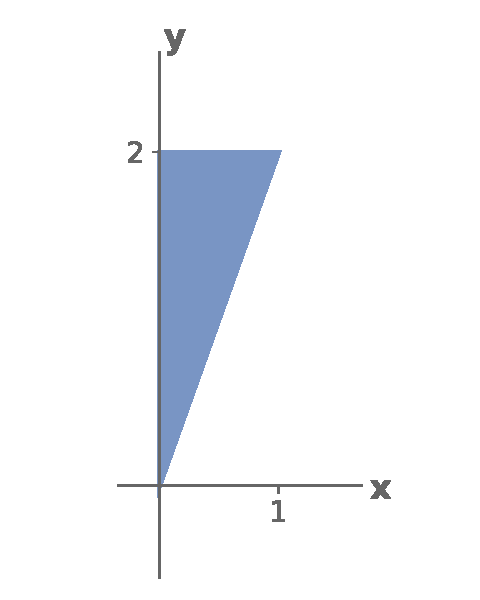
\includegraphics[width = 0.32\linewidth]{triangular_region}
    \answer{The slanted edge is the line $y = 2x$. Integrating $y$ first:
    $\int_0^1\!\!\int_{2x}^{2} (x-y)\,dy\,dx
     = \int_0^1 \left[xy - \tfrac{y^2}{2}\right]_{2x}^{2} dx
     = \int_0^1 (2x - 2)\,dx = -1$.
    (Integrating $x$ first, $\int_0^2\!\int_0^{y/2}(x-y)\,dx\,dy$, also gives
    $-1$.)}
  \end{enumerate}

  \item The point $P$ in the $x$-$y$ plane has Cartesian coordinates
        $x=-2,\ y=-2$. What are its polar coordinates $\rho$ and $\phi$?
        (You may have learned these as $r$ and $\theta$ --- they mean the
        same thing.)
  \answer{Draw it: $P$ is in the third quadrant.
  $\rho = \sqrt{(-2)^2 + (-2)^2} = 2\sqrt{2}$ and
  $\phi = \pi + \pi/4 = 5\pi/4$ (i.e.\ $225\degs$).}

  \item The plot below shows a function $f(x)$. On the axes provided at the
        right, sketch the function $df/dx$. Numbers are included on the
        horizontal axis, but you do not need to show numbers on the vertical
        axis.

  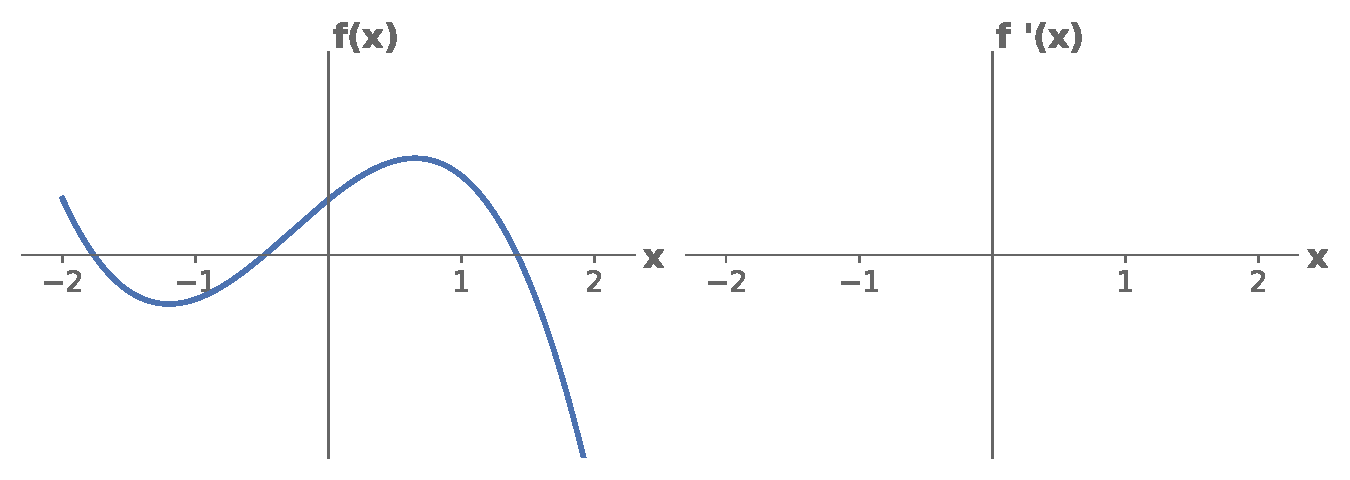
\includegraphics[width = \linewidth]{plotting_derivative}
  \answer{Where $f$ has its minimum (just before $x=-1$) and its maximum
  (between $0$ and $1$), $f' = 0$. To the left of the minimum and to the right
  of the maximum, $f$ is decreasing, so $f' < 0$; between them $f$ is
  increasing, so $f' > 0$. The sketch is a downward-opening arch crossing zero
  just before $x=-1$ and again between $0$ and $1$, negative and falling
  steeply at the right edge.}

  \item The plot below shows a cosine function $x(t)$.
  \begin{enumerate}[label = \alph*.]
    \item What are the amplitude $A$, period $T$, and angular frequency
          $\omega$?
    \item Write the function $x(t)$. {\em Hint: try plugging some points into
          your answer to make sure it matches the graph.}
  \end{enumerate}
  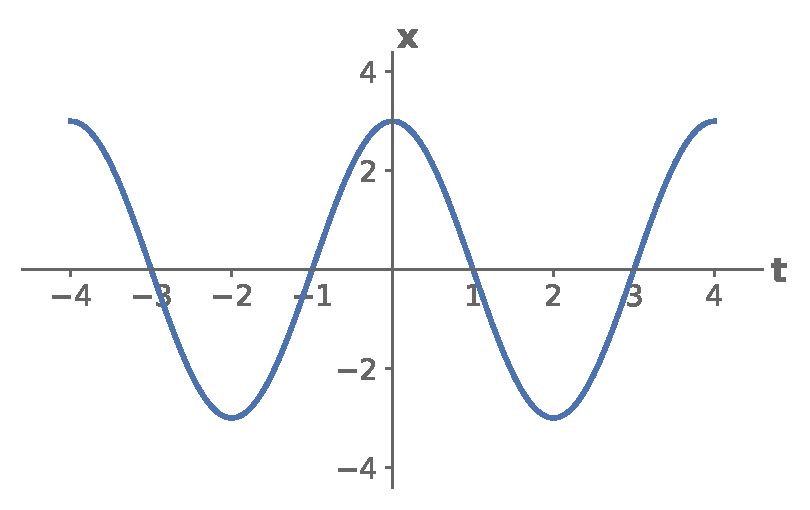
\includegraphics[width = 0.5\linewidth]{cosine_plot}
  \answer{$A = 3$ (the curve runs from $-3$ to $3$); $T = 4$ (peak to
  peak); $\omega = 2\pi/T = \pi/2$. So $x(t) = 3\cos(\pi t/2)$. Check:
  $x(0)=3$, $x(1)=0$, $x(2)=-3$, $x(4)=3$. \checkmark}

  \item The vector $\vA$ is given by
        $\vA = -2\hx + 5\hy$. The vector $\vB$ has magnitude $2\sqrt{2}$ and
        direction $30\degs$ clockwise from the positive $x$ axis.
  \begin{enumerate}[label = \alph*.]
    \item Find the magnitude and direction of $\vA$.
    \answer{$\abs{\vA} = \sqrt{4+25} = \sqrt{29}$. Draw it: $\vA$ points up
    and to the left, an angle $\tan^{-1}(2/5)$ counterclockwise from the
    positive $y$ axis (equivalently $\tan^{-1}(5/2)$ up from the negative $x$
    axis).}
    \item Find the components of $\vB$.
    \answer{$B_x = 2\sqrt{2}\cos(30\degs) = \sqrt{6}$,
    $B_y = -2\sqrt{2}\sin(30\degs) = -\sqrt{2}$ (negative: $30\degs$
    \emph{clockwise} is below the axis).}
    \item Find $\vA \cdot \vB$.
    \answer{$\vA\cdot\vB = A_x B_x + A_y B_y
    = -2\sqrt{6} - 5\sqrt{2}$. Sanity check: the vectors point mostly away
    from each other, so a negative answer makes sense.}
  \end{enumerate}

  \item An object is moving in some complicated way, and you want to solve
        for its acceleration at some particular moment. You can't actually do
        that calculation here, because we're not giving you enough
        information. Instead, check each of the following possible answers to
        determine whether it has correct units. Assume that:
  \begin{itemize}
    \item $F_{1}, F_{2}$, and so on are forces,
    \item $m$ is a mass,
    \item $D$ is a distance,
    \item $T$ is a time,
    \item $v_{0}$ and $v_{f}$ are speeds.
  \end{itemize}
  Which of the following possible answers have correct units? (There may be
  more than one option with correct units.)
  \begin{enumerate}[label = \alph*.]
    \item $a = \dfrac{v_{0} + v_{f}}{T}$
    \item $a = \dfrac{v_{0} + v_{f} + 1}{T}$
    \item $a = \dfrac{D}{T^{2}}$
    \item $a = \dfrac{D}{T^{2}}\,e^{-v_{f}/v_{0}}$
    \item $a = \dfrac{D}{T^{2}}\,e^{-v_{f}/(D T)}$
  \end{enumerate}
  \answer{Acceleration needs units of distance over time squared.
  (a) speed/time \checkmark\ YES.
  (b) NO --- you can't add a speed and the unitless number 1.
  (c) \checkmark\ YES.
  (d) the exponent is speed/speed, which is unitless, so \checkmark\ YES.
  (e) NO --- the exponent has units of $1/(\text{time})^2$, and exponents
  must be unitless.
  Correct units: a, c, and d.}
\end{enumerate}

\end{document}
"
%   master:  pdflatex -jobname=MathPretest-master MathPretest.tex
%
\documentclass[12pt]{article}
%%%%%%%%%%%%%%%%%%%%%%%%%%%%%%%%%%%%%%%%%%%%%%%%%%%%%%%%%%%%%
\input{../../macros}
%%%%%%%%%%%%%%%%%%%%%%%%%%%%%%%%%%%%%%%%%%%%%%%%%%%%%%%%%%%%%
% macros.tex defaults to \mastertrue; a student build passes \STUDENTVERSION.
\ifdefined\STUDENTVERSION \masterfalse \else \mastertrue \fi

\usepackage{graphicx}
\usepackage{enumitem}
\newcommand{\degs}{^{\circ}}
% macros.tex makes top-level enumerates lettered; this doc numbers its
% problems 1-9 with lettered subparts.
\renewcommand{\labelenumi}{\arabic{enumi}.}

\pagestyle{empty}
\begin{document}

\begin{center}
{\bf PHY 210: Mathematical Methods of Physical Sciences and Engineering\\
Smith College, Fall 2026}
\end{center}

\setlength{\unitlength}{1in}
\begin{picture}(6,.1)
\put(0,0) {\line(1,0){6.25}}
\end{picture}

\vskip.15in
\begin{center}
{\Large \bf Math Pretest}\\[2pt]
% Due date confirmed 2026-09-02 against the F2026 calendar (EXTRA_DUE) and
% the Moodle assignment: Fri Sep 18, 22:00. Same Friday as WHW02, as in S26.
{Due: Friday, September 18, end of day}
\end{center}

\subsection*{Instructions}
Set aside two hours for this pretest.

Please don't use a calculator, a computer, or any references. This pretest is
meant to give both of us a clear picture of which areas you should practice
more, so it won't help you to look things up. It is graded for completion, not
correctness: doing it thoughtfully is what earns the credit.

Give your answers as expressions. For example, if your final answer to a
question is $\sqrt{10}$, you should leave it as $\sqrt{10}$. If you have
something that can easily be simplified, like $e^{0}$ or $\ln(1)$, you should
simplify it.

\begin{enumerate}
  \item Write the equation of a line with slope $-5$ that passes through the
        point $(-2,2)$.
  \answer{Point-slope form: $y - 2 = -5(x+2)$, i.e.\ $y = -5x - 8$.
  Check: $x=-2$ gives $y=2$. \checkmark}

  \item Find the slope and concavity of $f(x) = x^{3} - x$ at $x=2$.
  \answer{$f'(x) = 3x^2 - 1$ and $f''(x) = 6x$, so at $x=2$ the slope is
  $f'(2) = 11$ and the concavity is $f''(2) = 12$ (concave up).}

  \item Calculate the following derivatives:
  \begin{enumerate}[label = \alph*.]
    \item $\pd{f}{y}$ for $f(x,y) = e^{3 x \sin(ky)}$
    \answer{$\pd{f}{y} = 3kx\cos(ky)\, e^{3x\sin(ky)}$.}
    \item $\fd{f}{t}$ for $f(x,y) = x^{3}e^{y}$, with $x(t) = \cos(2t)$ and
          $y(t) = t^{2} + 1$
    \answer{Chain rule:
    $\fd{f}{t} = \pd{f}{x}\fd{x}{t} + \pd{f}{y}\fd{y}{t}
               = 3x^2 e^y \left(-2\sin 2t\right) + x^3 e^y (2t)
               = 2t\cos^3(2t)\,e^{t^2+1} - 6\sin(2t)\cos^2(2t)\,e^{t^2+1}$.}
  \end{enumerate}

  \item Evaluate the following integrals:
  \begin{enumerate}[label = \alph*.]
    \item $\displaystyle\int \sin(x)\, [2 \cos(x) + 3]^{5}\,dx$
    \answer{Let $u = 2\cos x + 3$, $du = -2\sin x\,dx$:
    $-\tfrac{1}{2}\int u^5\,du = -\tfrac{1}{12}(2\cos x + 3)^6 + C$.}
    \item Integrate $f(x,y) = x-y$ over the triangular region shown below.

    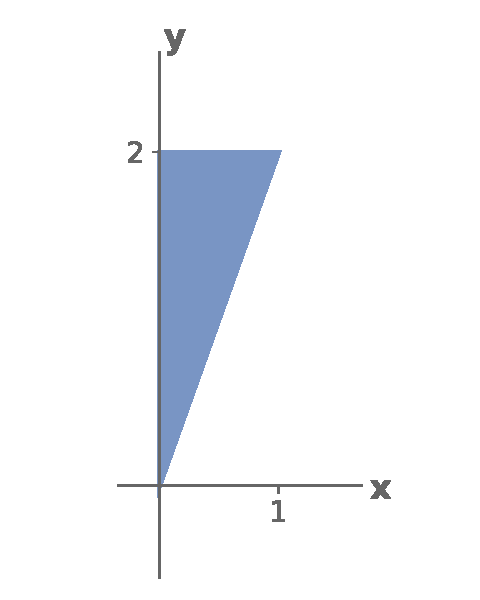
\includegraphics[width = 0.32\linewidth]{triangular_region}
    \answer{The slanted edge is the line $y = 2x$. Integrating $y$ first:
    $\int_0^1\!\!\int_{2x}^{2} (x-y)\,dy\,dx
     = \int_0^1 \left[xy - \tfrac{y^2}{2}\right]_{2x}^{2} dx
     = \int_0^1 (2x - 2)\,dx = -1$.
    (Integrating $x$ first, $\int_0^2\!\int_0^{y/2}(x-y)\,dx\,dy$, also gives
    $-1$.)}
  \end{enumerate}

  \item The point $P$ in the $x$-$y$ plane has Cartesian coordinates
        $x=-2,\ y=-2$. What are its polar coordinates $\rho$ and $\phi$?
        (You may have learned these as $r$ and $\theta$ --- they mean the
        same thing.)
  \answer{Draw it: $P$ is in the third quadrant.
  $\rho = \sqrt{(-2)^2 + (-2)^2} = 2\sqrt{2}$ and
  $\phi = \pi + \pi/4 = 5\pi/4$ (i.e.\ $225\degs$).}

  \item The plot below shows a function $f(x)$. On the axes provided at the
        right, sketch the function $df/dx$. Numbers are included on the
        horizontal axis, but you do not need to show numbers on the vertical
        axis.

  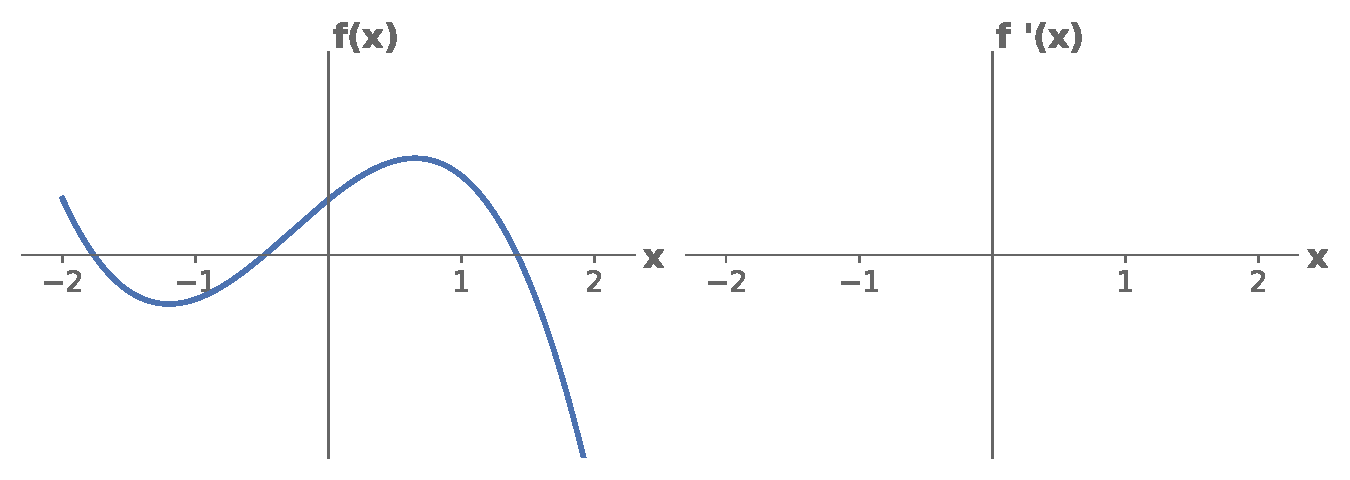
\includegraphics[width = \linewidth]{plotting_derivative}
  \answer{Where $f$ has its minimum (just before $x=-1$) and its maximum
  (between $0$ and $1$), $f' = 0$. To the left of the minimum and to the right
  of the maximum, $f$ is decreasing, so $f' < 0$; between them $f$ is
  increasing, so $f' > 0$. The sketch is a downward-opening arch crossing zero
  just before $x=-1$ and again between $0$ and $1$, negative and falling
  steeply at the right edge.}

  \item The plot below shows a cosine function $x(t)$.
  \begin{enumerate}[label = \alph*.]
    \item What are the amplitude $A$, period $T$, and angular frequency
          $\omega$?
    \item Write the function $x(t)$. {\em Hint: try plugging some points into
          your answer to make sure it matches the graph.}
  \end{enumerate}
  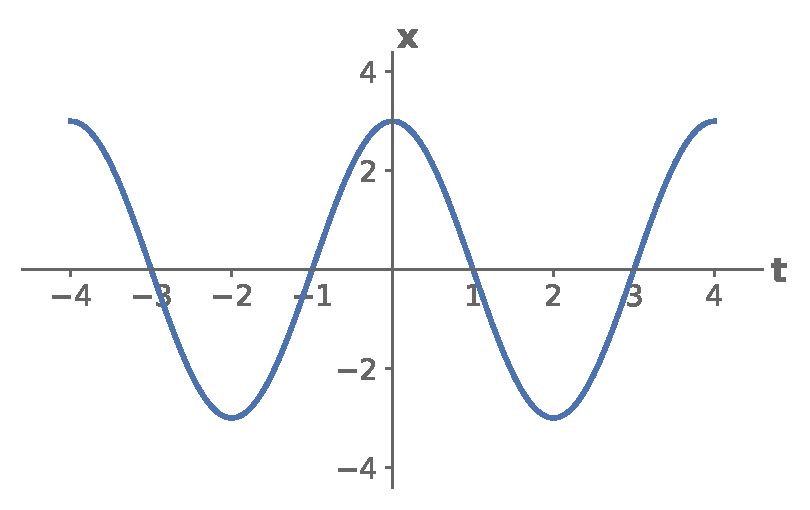
\includegraphics[width = 0.5\linewidth]{cosine_plot}
  \answer{$A = 3$ (the curve runs from $-3$ to $3$); $T = 4$ (peak to
  peak); $\omega = 2\pi/T = \pi/2$. So $x(t) = 3\cos(\pi t/2)$. Check:
  $x(0)=3$, $x(1)=0$, $x(2)=-3$, $x(4)=3$. \checkmark}

  \item The vector $\vA$ is given by
        $\vA = -2\hx + 5\hy$. The vector $\vB$ has magnitude $2\sqrt{2}$ and
        direction $30\degs$ clockwise from the positive $x$ axis.
  \begin{enumerate}[label = \alph*.]
    \item Find the magnitude and direction of $\vA$.
    \answer{$\abs{\vA} = \sqrt{4+25} = \sqrt{29}$. Draw it: $\vA$ points up
    and to the left, an angle $\tan^{-1}(2/5)$ counterclockwise from the
    positive $y$ axis (equivalently $\tan^{-1}(5/2)$ up from the negative $x$
    axis).}
    \item Find the components of $\vB$.
    \answer{$B_x = 2\sqrt{2}\cos(30\degs) = \sqrt{6}$,
    $B_y = -2\sqrt{2}\sin(30\degs) = -\sqrt{2}$ (negative: $30\degs$
    \emph{clockwise} is below the axis).}
    \item Find $\vA \cdot \vB$.
    \answer{$\vA\cdot\vB = A_x B_x + A_y B_y
    = -2\sqrt{6} - 5\sqrt{2}$. Sanity check: the vectors point mostly away
    from each other, so a negative answer makes sense.}
  \end{enumerate}

  \item An object is moving in some complicated way, and you want to solve
        for its acceleration at some particular moment. You can't actually do
        that calculation here, because we're not giving you enough
        information. Instead, check each of the following possible answers to
        determine whether it has correct units. Assume that:
  \begin{itemize}
    \item $F_{1}, F_{2}$, and so on are forces,
    \item $m$ is a mass,
    \item $D$ is a distance,
    \item $T$ is a time,
    \item $v_{0}$ and $v_{f}$ are speeds.
  \end{itemize}
  Which of the following possible answers have correct units? (There may be
  more than one option with correct units.)
  \begin{enumerate}[label = \alph*.]
    \item $a = \dfrac{v_{0} + v_{f}}{T}$
    \item $a = \dfrac{v_{0} + v_{f} + 1}{T}$
    \item $a = \dfrac{D}{T^{2}}$
    \item $a = \dfrac{D}{T^{2}}\,e^{-v_{f}/v_{0}}$
    \item $a = \dfrac{D}{T^{2}}\,e^{-v_{f}/(D T)}$
  \end{enumerate}
  \answer{Acceleration needs units of distance over time squared.
  (a) speed/time \checkmark\ YES.
  (b) NO --- you can't add a speed and the unitless number 1.
  (c) \checkmark\ YES.
  (d) the exponent is speed/speed, which is unitless, so \checkmark\ YES.
  (e) NO --- the exponent has units of $1/(\text{time})^2$, and exponents
  must be unitless.
  Correct units: a, c, and d.}
\end{enumerate}

\end{document}
"
%   master:  pdflatex -jobname=MathPretest-master MathPretest.tex
%
\documentclass[12pt]{article}
%%%%%%%%%%%%%%%%%%%%%%%%%%%%%%%%%%%%%%%%%%%%%%%%%%%%%%%%%%%%%
\input{../../macros}
%%%%%%%%%%%%%%%%%%%%%%%%%%%%%%%%%%%%%%%%%%%%%%%%%%%%%%%%%%%%%
% macros.tex defaults to \mastertrue; a student build passes \STUDENTVERSION.
\ifdefined\STUDENTVERSION \masterfalse \else \mastertrue \fi

\usepackage{graphicx}
\usepackage{enumitem}
\newcommand{\degs}{^{\circ}}
% macros.tex makes top-level enumerates lettered; this doc numbers its
% problems 1-9 with lettered subparts.
\renewcommand{\labelenumi}{\arabic{enumi}.}

\pagestyle{empty}
\begin{document}

\begin{center}
{\bf PHY 210: Mathematical Methods of Physical Sciences and Engineering\\
Smith College, Fall 2026}
\end{center}

\setlength{\unitlength}{1in}
\begin{picture}(6,.1)
\put(0,0) {\line(1,0){6.25}}
\end{picture}

\vskip.15in
\begin{center}
{\Large \bf Math Pretest}\\[2pt]
% Due date confirmed 2026-09-02 against the F2026 calendar (EXTRA_DUE) and
% the Moodle assignment: Fri Sep 18, 22:00. Same Friday as WHW02, as in S26.
{Due: Friday, September 18, end of day}
\end{center}

\subsection*{Instructions}
Set aside two hours for this pretest.

Please don't use a calculator, a computer, or any references. This pretest is
meant to give both of us a clear picture of which areas you should practice
more, so it won't help you to look things up. It is graded for completion, not
correctness: doing it thoughtfully is what earns the credit.

Give your answers as expressions. For example, if your final answer to a
question is $\sqrt{10}$, you should leave it as $\sqrt{10}$. If you have
something that can easily be simplified, like $e^{0}$ or $\ln(1)$, you should
simplify it.

\begin{enumerate}
  \item Write the equation of a line with slope $-5$ that passes through the
        point $(-2,2)$.
  \answer{Point-slope form: $y - 2 = -5(x+2)$, i.e.\ $y = -5x - 8$.
  Check: $x=-2$ gives $y=2$. \checkmark}

  \item Find the slope and concavity of $f(x) = x^{3} - x$ at $x=2$.
  \answer{$f'(x) = 3x^2 - 1$ and $f''(x) = 6x$, so at $x=2$ the slope is
  $f'(2) = 11$ and the concavity is $f''(2) = 12$ (concave up).}

  \item Calculate the following derivatives:
  \begin{enumerate}[label = \alph*.]
    \item $\pd{f}{y}$ for $f(x,y) = e^{3 x \sin(ky)}$
    \answer{$\pd{f}{y} = 3kx\cos(ky)\, e^{3x\sin(ky)}$.}
    \item $\fd{f}{t}$ for $f(x,y) = x^{3}e^{y}$, with $x(t) = \cos(2t)$ and
          $y(t) = t^{2} + 1$
    \answer{Chain rule:
    $\fd{f}{t} = \pd{f}{x}\fd{x}{t} + \pd{f}{y}\fd{y}{t}
               = 3x^2 e^y \left(-2\sin 2t\right) + x^3 e^y (2t)
               = 2t\cos^3(2t)\,e^{t^2+1} - 6\sin(2t)\cos^2(2t)\,e^{t^2+1}$.}
  \end{enumerate}

  \item Evaluate the following integrals:
  \begin{enumerate}[label = \alph*.]
    \item $\displaystyle\int \sin(x)\, [2 \cos(x) + 3]^{5}\,dx$
    \answer{Let $u = 2\cos x + 3$, $du = -2\sin x\,dx$:
    $-\tfrac{1}{2}\int u^5\,du = -\tfrac{1}{12}(2\cos x + 3)^6 + C$.}
    \item Integrate $f(x,y) = x-y$ over the triangular region shown below.

    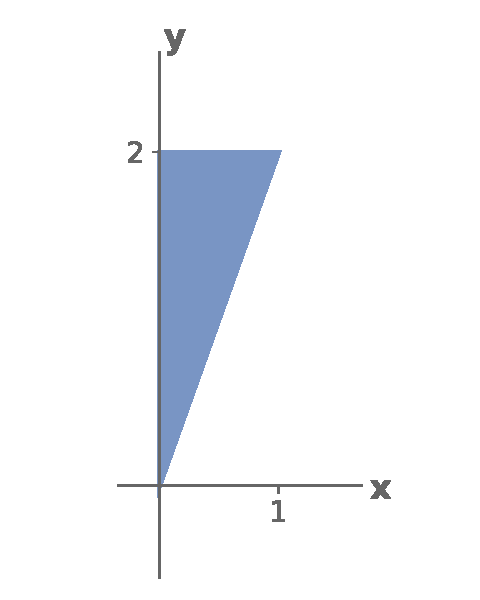
\includegraphics[width = 0.32\linewidth]{triangular_region}
    \answer{The slanted edge is the line $y = 2x$. Integrating $y$ first:
    $\int_0^1\!\!\int_{2x}^{2} (x-y)\,dy\,dx
     = \int_0^1 \left[xy - \tfrac{y^2}{2}\right]_{2x}^{2} dx
     = \int_0^1 (2x - 2)\,dx = -1$.
    (Integrating $x$ first, $\int_0^2\!\int_0^{y/2}(x-y)\,dx\,dy$, also gives
    $-1$.)}
  \end{enumerate}

  \item The point $P$ in the $x$-$y$ plane has Cartesian coordinates
        $x=-2,\ y=-2$. What are its polar coordinates $\rho$ and $\phi$?
        (You may have learned these as $r$ and $\theta$ --- they mean the
        same thing.)
  \answer{Draw it: $P$ is in the third quadrant.
  $\rho = \sqrt{(-2)^2 + (-2)^2} = 2\sqrt{2}$ and
  $\phi = \pi + \pi/4 = 5\pi/4$ (i.e.\ $225\degs$).}

  \item The plot below shows a function $f(x)$. On the axes provided at the
        right, sketch the function $df/dx$. Numbers are included on the
        horizontal axis, but you do not need to show numbers on the vertical
        axis.

  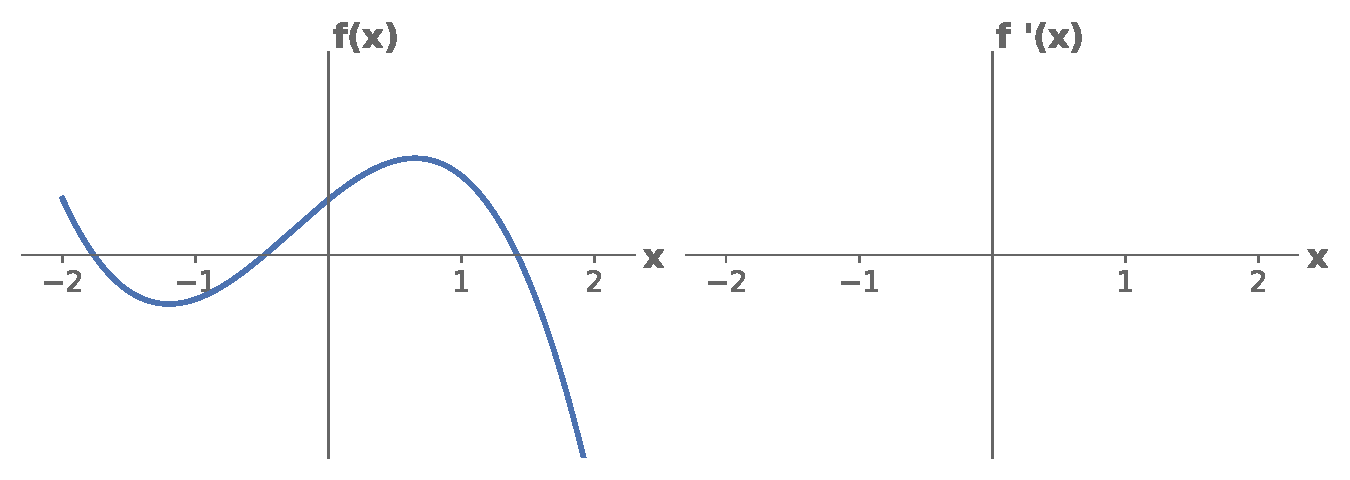
\includegraphics[width = \linewidth]{plotting_derivative}
  \answer{Where $f$ has its minimum (just before $x=-1$) and its maximum
  (between $0$ and $1$), $f' = 0$. To the left of the minimum and to the right
  of the maximum, $f$ is decreasing, so $f' < 0$; between them $f$ is
  increasing, so $f' > 0$. The sketch is a downward-opening arch crossing zero
  just before $x=-1$ and again between $0$ and $1$, negative and falling
  steeply at the right edge.}

  \item The plot below shows a cosine function $x(t)$.
  \begin{enumerate}[label = \alph*.]
    \item What are the amplitude $A$, period $T$, and angular frequency
          $\omega$?
    \item Write the function $x(t)$. {\em Hint: try plugging some points into
          your answer to make sure it matches the graph.}
  \end{enumerate}
  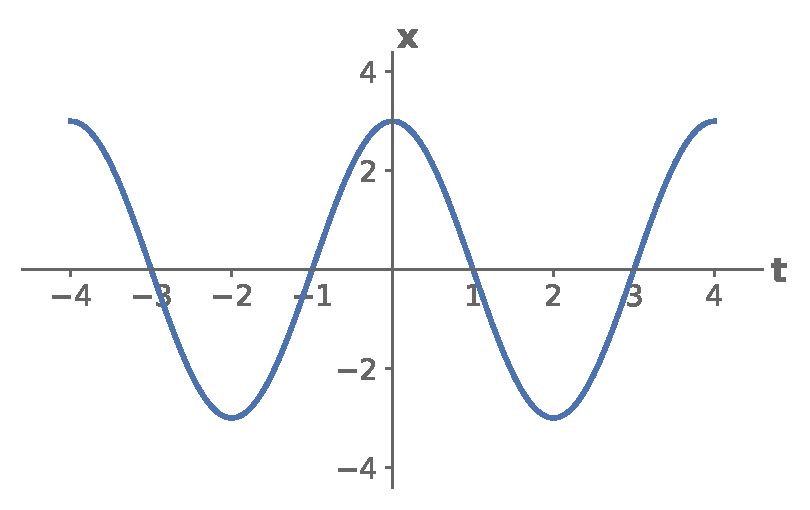
\includegraphics[width = 0.5\linewidth]{cosine_plot}
  \answer{$A = 3$ (the curve runs from $-3$ to $3$); $T = 4$ (peak to
  peak); $\omega = 2\pi/T = \pi/2$. So $x(t) = 3\cos(\pi t/2)$. Check:
  $x(0)=3$, $x(1)=0$, $x(2)=-3$, $x(4)=3$. \checkmark}

  \item The vector $\vA$ is given by
        $\vA = -2\hx + 5\hy$. The vector $\vB$ has magnitude $2\sqrt{2}$ and
        direction $30\degs$ clockwise from the positive $x$ axis.
  \begin{enumerate}[label = \alph*.]
    \item Find the magnitude and direction of $\vA$.
    \answer{$\abs{\vA} = \sqrt{4+25} = \sqrt{29}$. Draw it: $\vA$ points up
    and to the left, an angle $\tan^{-1}(2/5)$ counterclockwise from the
    positive $y$ axis (equivalently $\tan^{-1}(5/2)$ up from the negative $x$
    axis).}
    \item Find the components of $\vB$.
    \answer{$B_x = 2\sqrt{2}\cos(30\degs) = \sqrt{6}$,
    $B_y = -2\sqrt{2}\sin(30\degs) = -\sqrt{2}$ (negative: $30\degs$
    \emph{clockwise} is below the axis).}
    \item Find $\vA \cdot \vB$.
    \answer{$\vA\cdot\vB = A_x B_x + A_y B_y
    = -2\sqrt{6} - 5\sqrt{2}$. Sanity check: the vectors point mostly away
    from each other, so a negative answer makes sense.}
  \end{enumerate}

  \item An object is moving in some complicated way, and you want to solve
        for its acceleration at some particular moment. You can't actually do
        that calculation here, because we're not giving you enough
        information. Instead, check each of the following possible answers to
        determine whether it has correct units. Assume that:
  \begin{itemize}
    \item $F_{1}, F_{2}$, and so on are forces,
    \item $m$ is a mass,
    \item $D$ is a distance,
    \item $T$ is a time,
    \item $v_{0}$ and $v_{f}$ are speeds.
  \end{itemize}
  Which of the following possible answers have correct units? (There may be
  more than one option with correct units.)
  \begin{enumerate}[label = \alph*.]
    \item $a = \dfrac{v_{0} + v_{f}}{T}$
    \item $a = \dfrac{v_{0} + v_{f} + 1}{T}$
    \item $a = \dfrac{D}{T^{2}}$
    \item $a = \dfrac{D}{T^{2}}\,e^{-v_{f}/v_{0}}$
    \item $a = \dfrac{D}{T^{2}}\,e^{-v_{f}/(D T)}$
  \end{enumerate}
  \answer{Acceleration needs units of distance over time squared.
  (a) speed/time \checkmark\ YES.
  (b) NO --- you can't add a speed and the unitless number 1.
  (c) \checkmark\ YES.
  (d) the exponent is speed/speed, which is unitless, so \checkmark\ YES.
  (e) NO --- the exponent has units of $1/(\text{time})^2$, and exponents
  must be unitless.
  Correct units: a, c, and d.}
\end{enumerate}

\end{document}
